\def\x{x}
\def\Q{Q}
\def\bds#1{#1}
\def\tts#1{\texttt{\small #1}}

\section{Experiments}
\label{sec:thesims}

We perform both synthetic and real data experiments.

\subsection{Simulations}
We first illustrate our methods using a simulation of the model
\begin{equation}\nonumber
         Y_i = f_0(\x_{iS}) + \epsilon_i \quad (i=1,2,\ldots,n).
\end{equation}
Here $\x_{i}$ denotes data sample $i$ drawn from some distribution
$P$, and $f_0$ is the true regression function. The variables
$\x_{iS}$ are a subset of $\x_i$ with dimension $|S|=s$, where $S$
represents the set of relevant variables, and $\epsilon_i$ is additive
noise drawn from $\mathcal{N}(0,\sigma^2)$. For all simulations, we set
$\sigma^2$ so that the signal-to-noise ratio(SNR,
$\frac{\trm{std}(Y)}{\sigma}$) is 5. Also, for all simulations except
the sixth, we choose the set of relevant variables $S$ uniformly at
random among all variables $\{1,...,p\}$.

We study both the independent case where $P = N(0, I_p)$ and the
correlated case where $P$ is a correlated Gaussian Copula modified
slightly to satisfy the boundary flatness condition. We measure the
probability of exact selection in the independent case and the
probability of screening in the correlated case. We also study both
cases where the regression function is parametric (quadratic) and
cases where the regression function is nonparametric (softmax of
linear forms). In all our experiments, we mark a variable as selected
if either the AC estimate $\| \hat{f}_j \|_\infty$ or the DC estimate
$\| \hat{g}_k \|_\infty$ is larger than $10^{-6}$. We set $\lambda =
0.5 \sqrt{\frac{\log^2 np}{n}}$ for all the simulations.

For the first three simulations, we use a quadratic form as the true regression function,
\[
f_0(x_{iS}) = x_{iS}^\tran \Q x_{iS}.
\]
The matrix $\Q$ is a symmetric positive definite matrix of dimension $s \times{} s$. 
Note that if $\Q$ is diagonal, then the true function is convex
additive; 
otherwise the true function is convex but not additive.

\subsubsection{First simulation}
In the \textrm{first simulation} (Figure~\ref{Support}a), we vary the
ambient dimension $p$. We set $Q$ to be one on the diagonal and $1/2$ on
the off-diagonal with $0.5$ probability, set $s=5$, and $p=64,128,256$
and $512$. We draw $X \sim N(0, I_p)$.  For each $(n,p)$ combination,
we generate $100$ independent trials.  In Figure~\ref{Support}(a), we
plot the probability of exact support recovery. We observe that the
algorithm performs consistent variable selection even if the
dimensionality is large. To give the reader a sense of the running
speed, for a dataset with $n=1,000$ and $p=512$, the code runs in
roughly two minutes on a machine with a 2.3 GHz Intel Core i5 CPU and 4
GB memory.


\subsubsection{Second simulation}
In the \textrm{second simulation} (Figure~\ref{Support}b,c), we vary the sparsity of the $Q$ matrix, that is, we vary the extent to which the true function is non-additive. We generate four $\Q$ matrices
plotted in Figure \ref{Support}(c), where the diagonal elements are all one and
the off-diagonal elements are $\frac{1}{2}$ with probability $\alpha$
($\alpha=0,0.2,0.5,1$ for the four cases). We show the 4 $\Q$ matrices we used in Figure~\ref{Support}(c).
We fix $p=128$, $s=5$, and $X \sim N(0,I_p)$.  We again run the AC/DC optimization on $100$
independent trials and plot the probability of exact recovery
in Figure \ref{Support}(b). The results demonstrate that AC/DC performs
consistent variable selection even if the true function is not additive (but
still convex). 

In the third, fourth, and fifth simulation, we use a correlated design. We generate $X$ from a non-Gaussian boundary flat distribution with covariance $\Sigma$. The distribution we used is a mixture of a uniform distribution and a Gaussian Copula.
\[
X \sim \gamma U([-2, 2]^p) + (1-\gamma) \trm{Copula}(0, \Sigma, F)
\]
The Gaussian Copula is a way to customize the marginal distributions of a Gaussian random variable while maintaining the same covariance. Gaussian Copula results when one applies a monotone transformation $F^{-1} \Phi$ onto each of the variables of a Gaussian random vector where $\Phi$ is the normal CDF and $F$ is the CDF of the new marginal distribution. In all our experiments, we set $\gamma = 0.05$ and set the marginal CDF $F$ so that marginal density of the Copula is bimodal and supported on $[-1.8, 1.8]$. The resulting marginal density of the mixture is shown in Figure~\ref{fig:copula_marginal}. Notice that boundary flatness holds because the distribution is uniform in the boundary area $[-2,2]^p \backslash [-1.8, 1.8]^p$.

\begin{figure*}
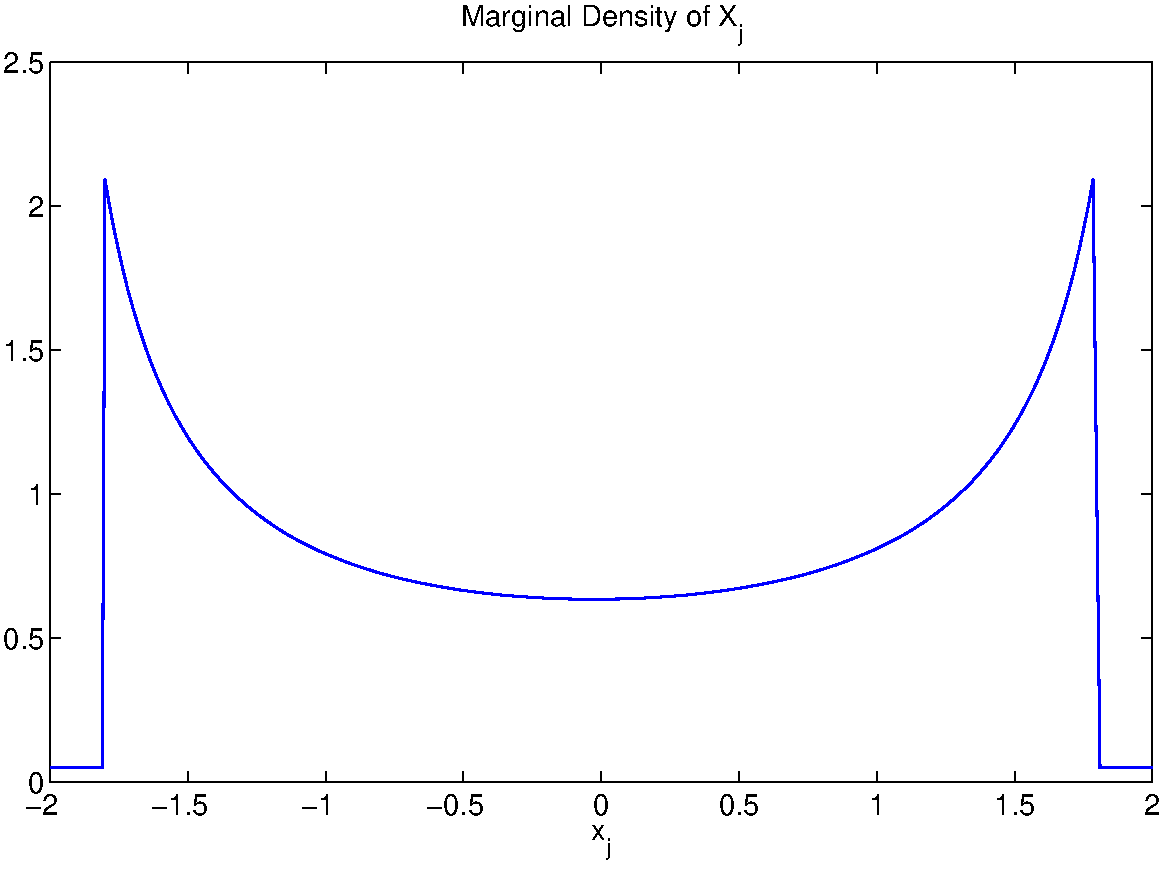
\includegraphics[width=.4\textwidth]{figs/copula_marginal}
\caption{Marginal density of the Gaussian Copula and Uniform Mixture}
\label{fig:copula_marginal}
\end{figure*}

\subsubsection{Third simulation}
In the \textrm{third simulation} (Figure~\ref{Support}d,e), we use the non-Gaussian distribution described above and set the covariance $\Sigma_{ij}=\nu^{|i-j|}$ for $\nu = 0, 0.2, 0.5, 0.9$. We use the non-additive $\Q$, same as in the first experiment, with $\alpha=0.5$ and fix $p=128, s=5$. We measure success not through exact recovery but through faithful recovery. We say that a trial is a successful if (1) all relevant variables were recovered and (2) fewer than $20$ variables were marked as relevant overall (true sparsity $s=5$). We use the same $\lambda$ as before. The probabilities of success are computed from 40 independent trials and plotted against various values of $\nu$ in Figure~\ref{Support}(d). Additionally, for $\nu = 0.5$, we show the number of selected variables versus the sample size as a box-and-whisker plot in Figure~\ref{Support}(e). As seen, for small to moderate correlations, AC/DC can successfully recover the relevant variables with only a small number of false positives. 

In the fourth and fifth simulation, we use a softmax function as the ground truth
\begin{align}
f_0(x_{iS}) = \log \left( \sum_{k=1}^K \exp( \beta_k^\tran x_{iS} ) \right) - \mu
\end{align}
We generate random unit vectors as $\{\beta_k \in \R^s\}_{k=1,...,K}$ and choose $\mu$ so that $f_0$ has mean-zero. We set $K = 7$ for all the experiments. 

\subsubsection{Fourth simulation}
For the \textrm{fourth simulation} (Figure~\ref{Support}f,g), we let $f_0$ be the softmax function and let $X$ be drawn from the boundary flat mixture distribution described earlier with the Toeplitz covariance $\Sigma_{ij}=\nu^{|i-j|}$ for $\nu = 0.5$. We set $s=5$ and vary $p=128,256,512$. We use the same faithful recovery criteria as the third simulation and plot the probability of faithful recovery against the number of samples in Figure~\ref{Support}(f). The probabilities are computed over 30 independent trials. Also, for $p=256$, we show the number of selected variables versus the sample size as a box-and-whisker plot in Figure~\ref{Support}(g). The softmax function is more challenging to estimate than the quadratic function; the softmax function requires about $n > 1500$ to achieve the same success probability as the quadratic function with $n=1000$. Regardless, we see that increasing the ambient dimension $p$ does not significantly affect the recovery probability.

%For the \textbf{fifth experiment} (Figure~\ref{Support}h), we vary the true sparsity level $s$. We let $f_0$ be the softmax function, $X \sim N(0, I)$, and set $p=128$. We compute the probability of exact recovery over 40 independent trials and plot the results in Figure~\ref{Support}(h).  

\subsubsection{Fifth simulation}
For the \textrm{fifth simulation} (Figure~\ref{fig:ac_v_dc}), we compare the variables selected via the AC stage and the variables selected via the DC stage. We use the softmax regression function and $X$ drawn from the boundary flat mixture distribution with a Toeplitz covariance and correlation level $\nu = -0.7$. We set $s=5, n=500, p=128$. We perform 30 independent trials and plot the frequency of variable selection in Figure~\ref{fig:ac_v_dc}. The true variables are $X_j$ for $j=5,6,7,8,9,10$. We plot the frequency of selection among only the first 20 variables, that is, $X_j$ for $j=1,...,20$. We do not plot selection frequencies for variables 21 to 128 because they are almost never selected by either AC or DC. As can be seen, the DC stage is slightly helpful in recovering the true variables but its effect is not significant. We thus believe that the DC stage, though important in theory, is not as important in practice; it may be omitted without significant detriment to the overall result. 

\begin{figure*}[!t]
\begin{center}
\begin{tabular}{cc}
%\hskip-10pt
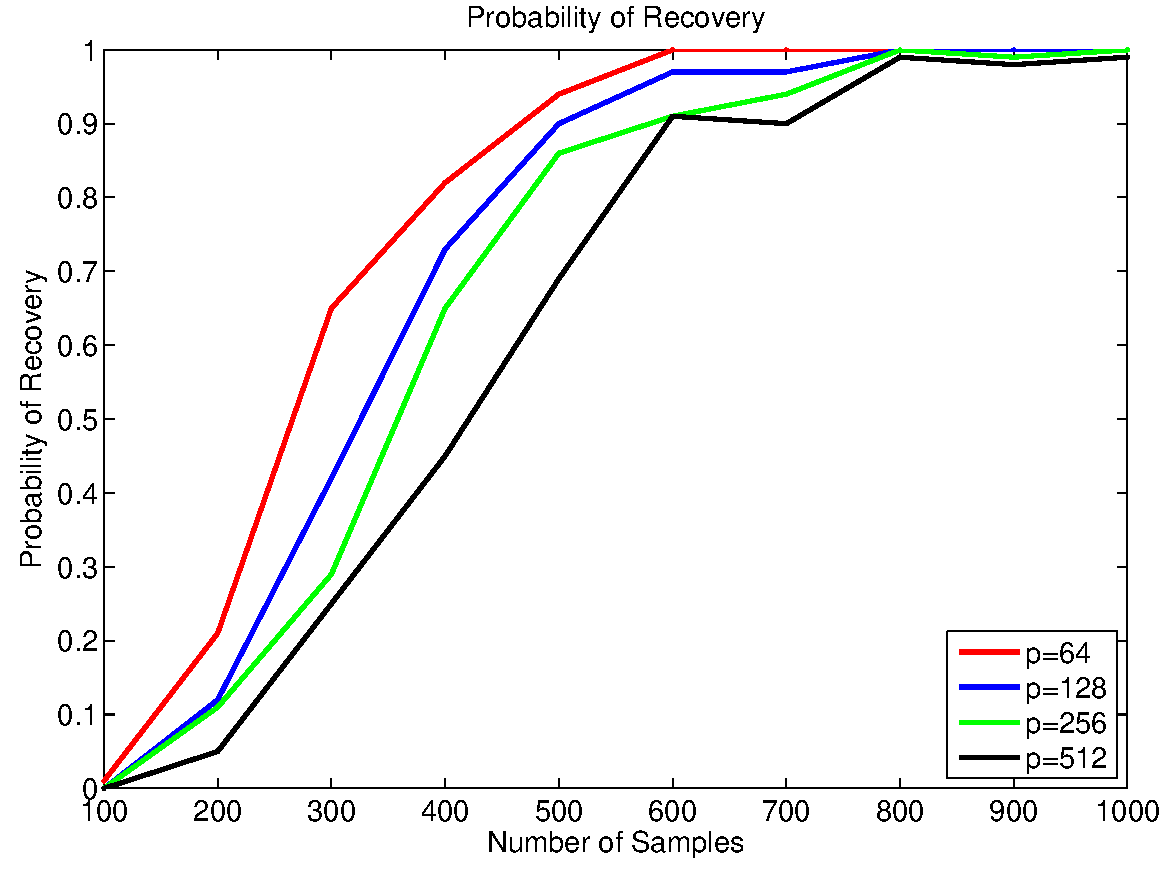
\includegraphics[width=.42\textwidth]{figs/CurveT} &
%\hskip-10pt
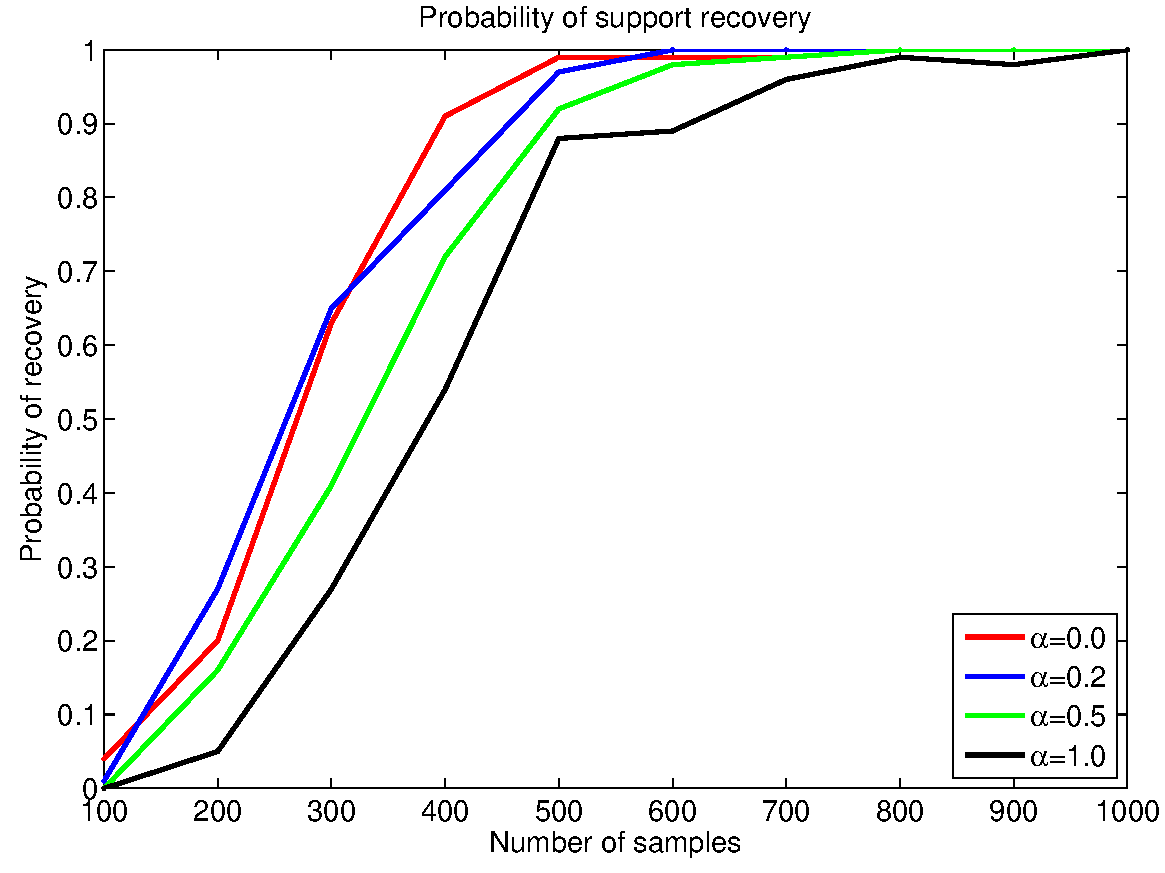
\includegraphics[width=.42\textwidth]{figs/CurveR} \\
(a) quadratic $f_0$, independent $X$, varying $p$  & (b) quadratic $f_0$, independent $X$, varying $\Q$ \\
%\hskip-10pt
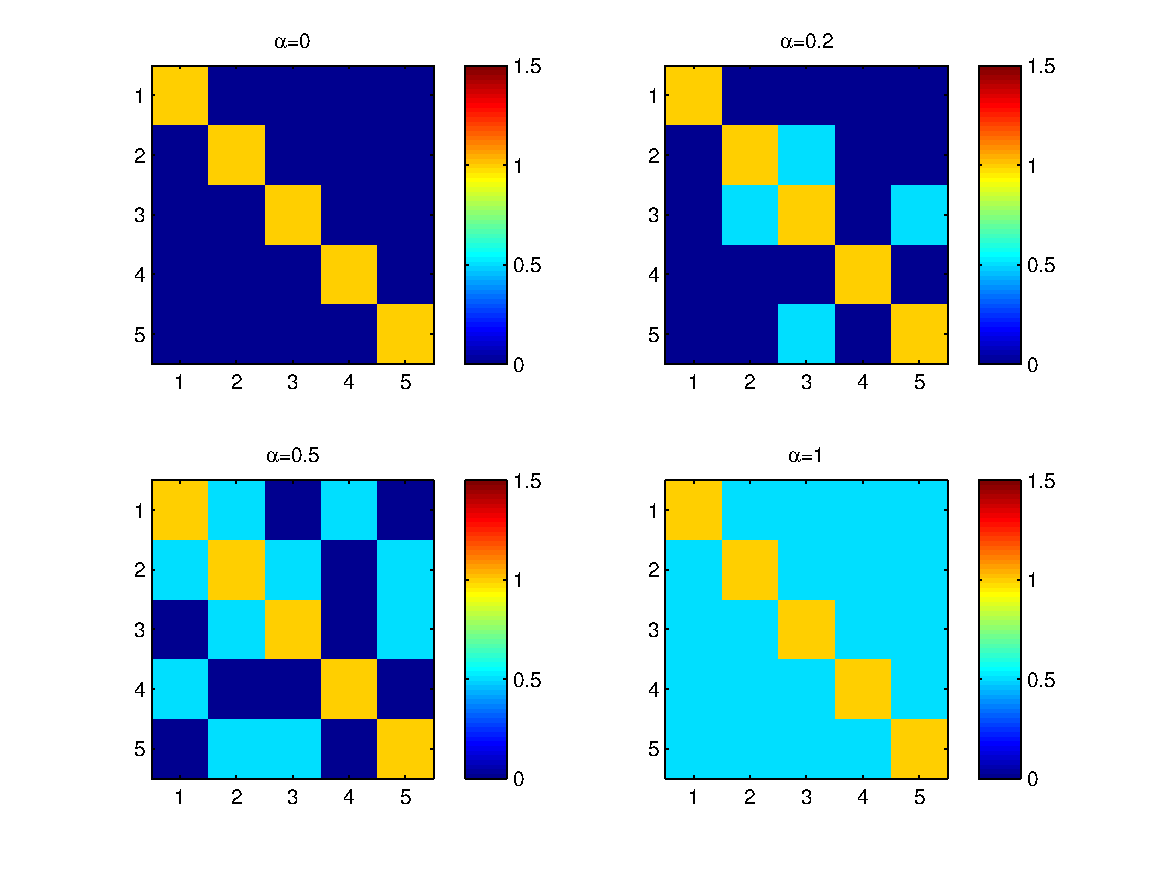
\includegraphics[width=.42\textwidth]{figs/Q} &
%\hskip-10pt
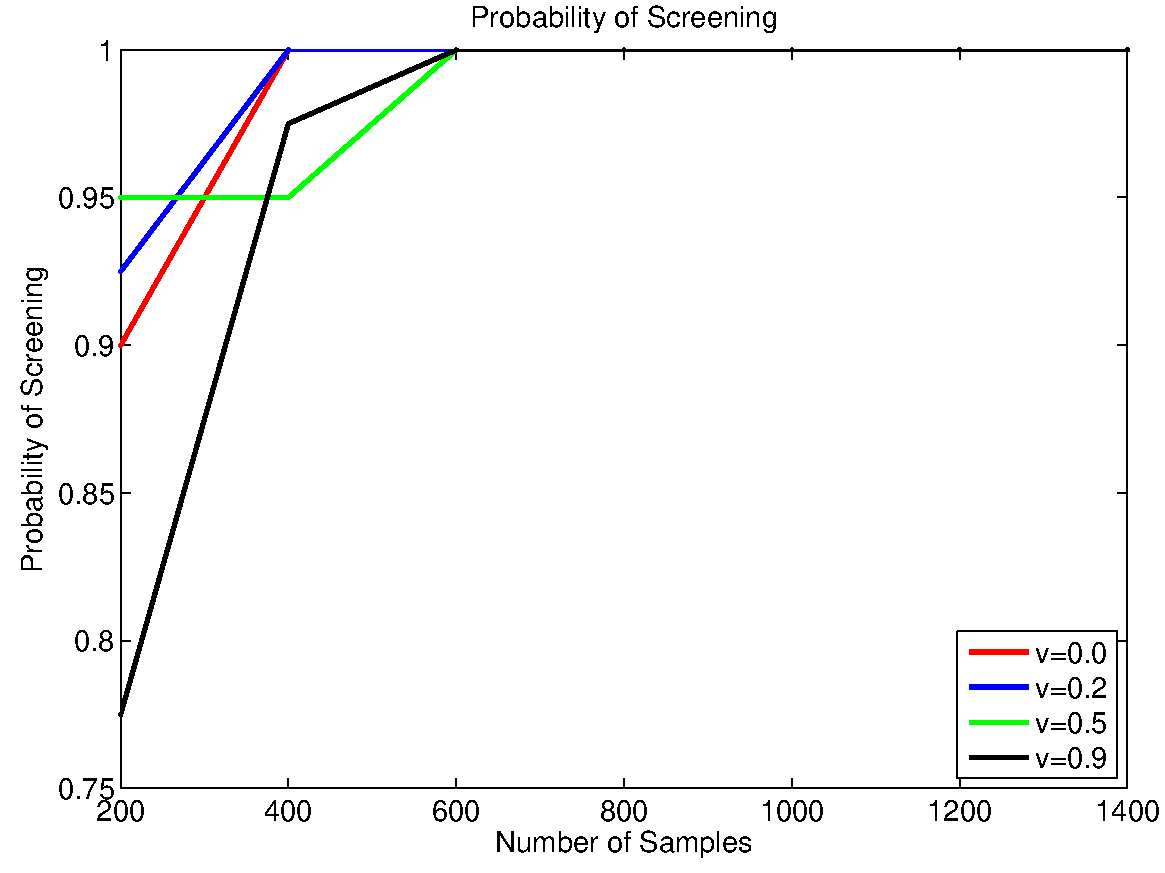
\includegraphics[width=.42\textwidth]{figs/CurveC}  \\
(c) four $\Q$ matrices used in (b) & (d) quadratic $f_0$, correlated $X$, varying correlation $\nu$ \\
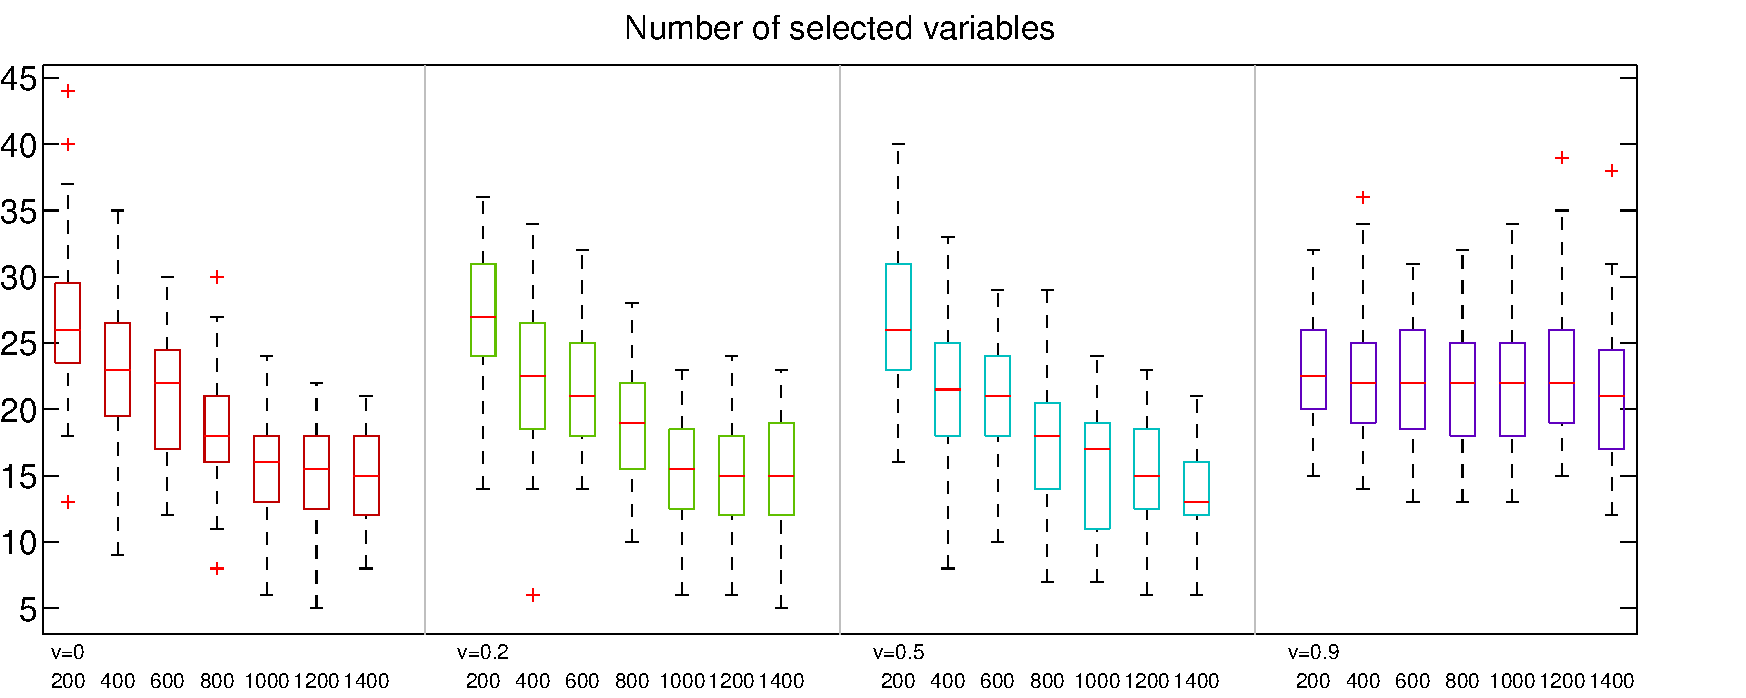
\includegraphics[width=.42\textwidth]{figs/C_support_box} & 
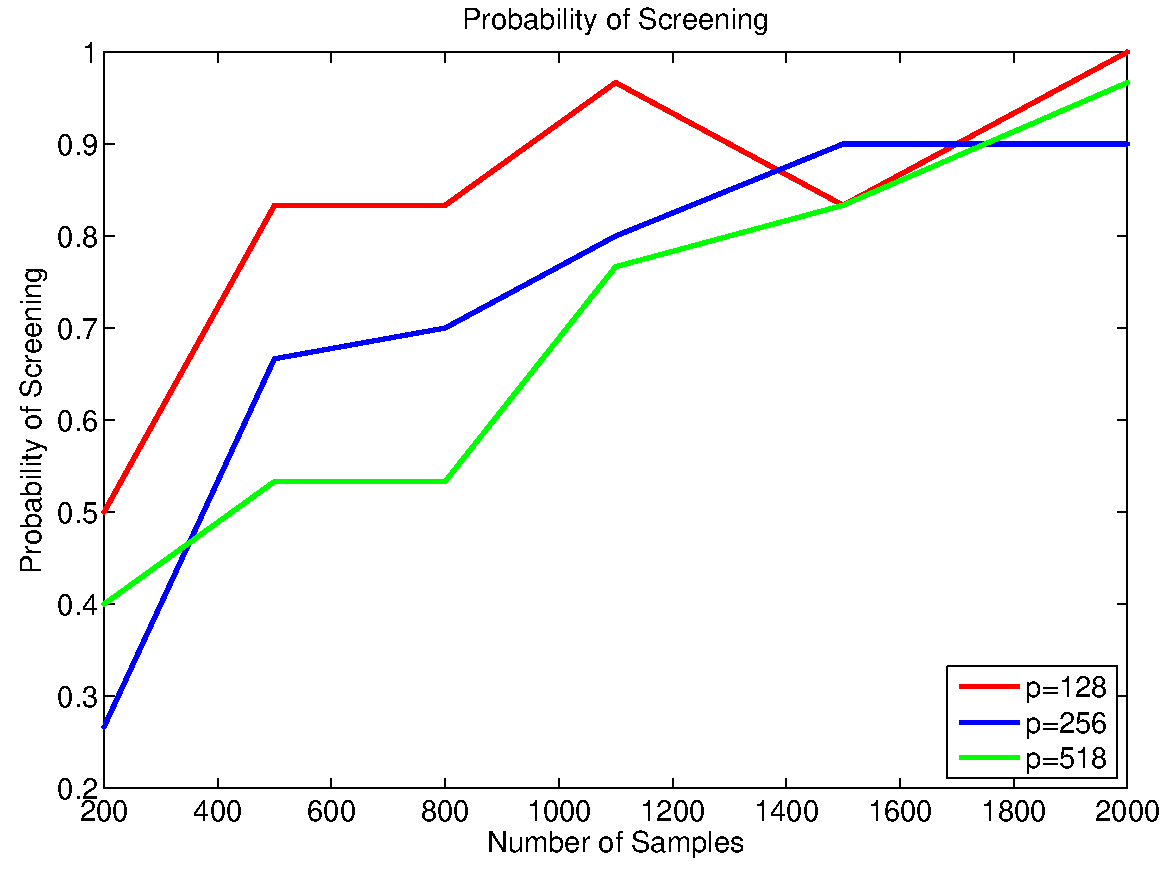
\includegraphics[width=.42\textwidth]{figs/CurveS}\\
(e) recovered support size for $\nu=0.5$ in (d) & (f) softmax $f_0$, correlated $X$, varying $p$ \\
%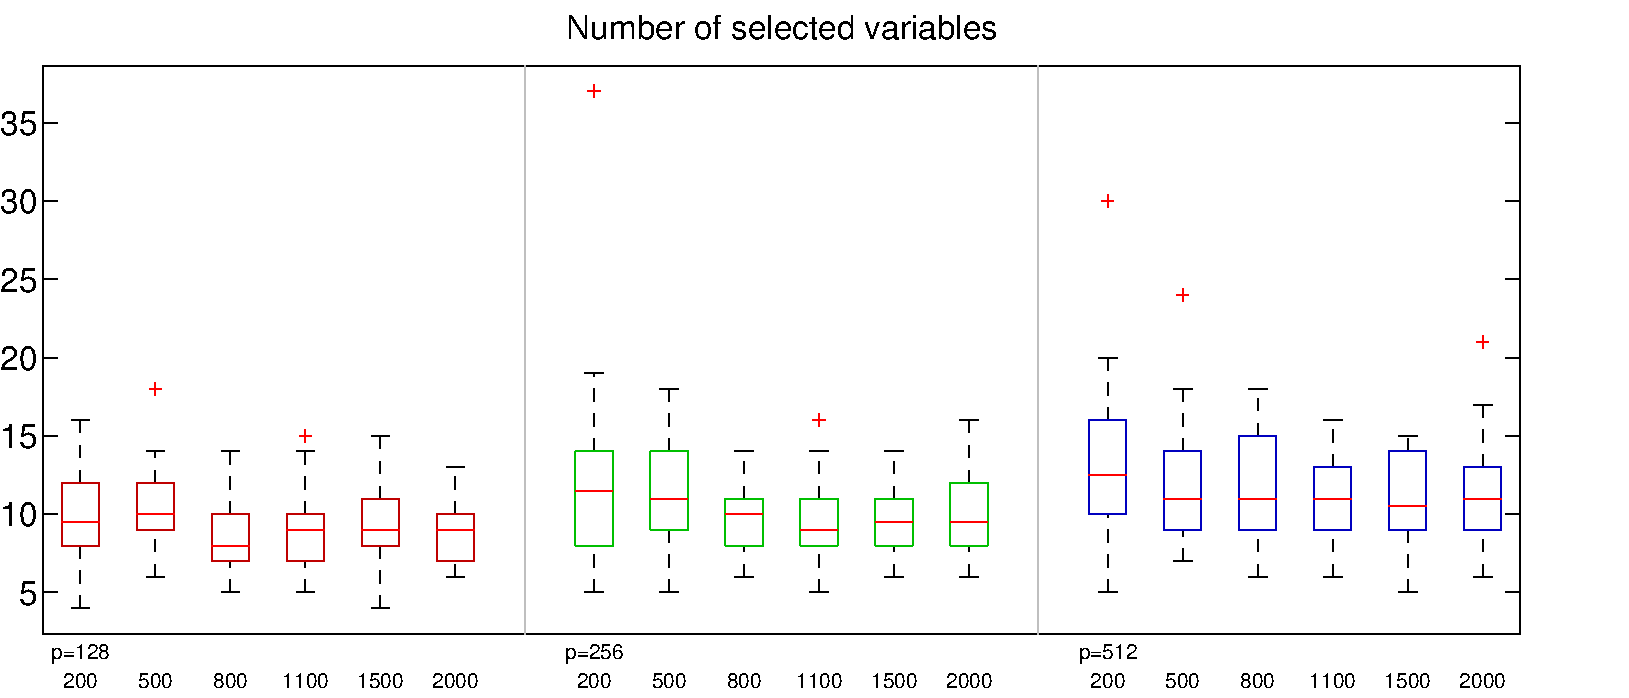
\includegraphics[width=0.42\textwidth]{figs/S_support_box} & \\
%(g) recovered support size for $p=256$ in (f) & (h) softmax $f_0$, correlated $X$, varying $s$ 
\end{tabular}
\end{center}
\caption{Support recovery results.}
\label{Support}
\vskip10pt
\end{figure*}

\begin{figure*}
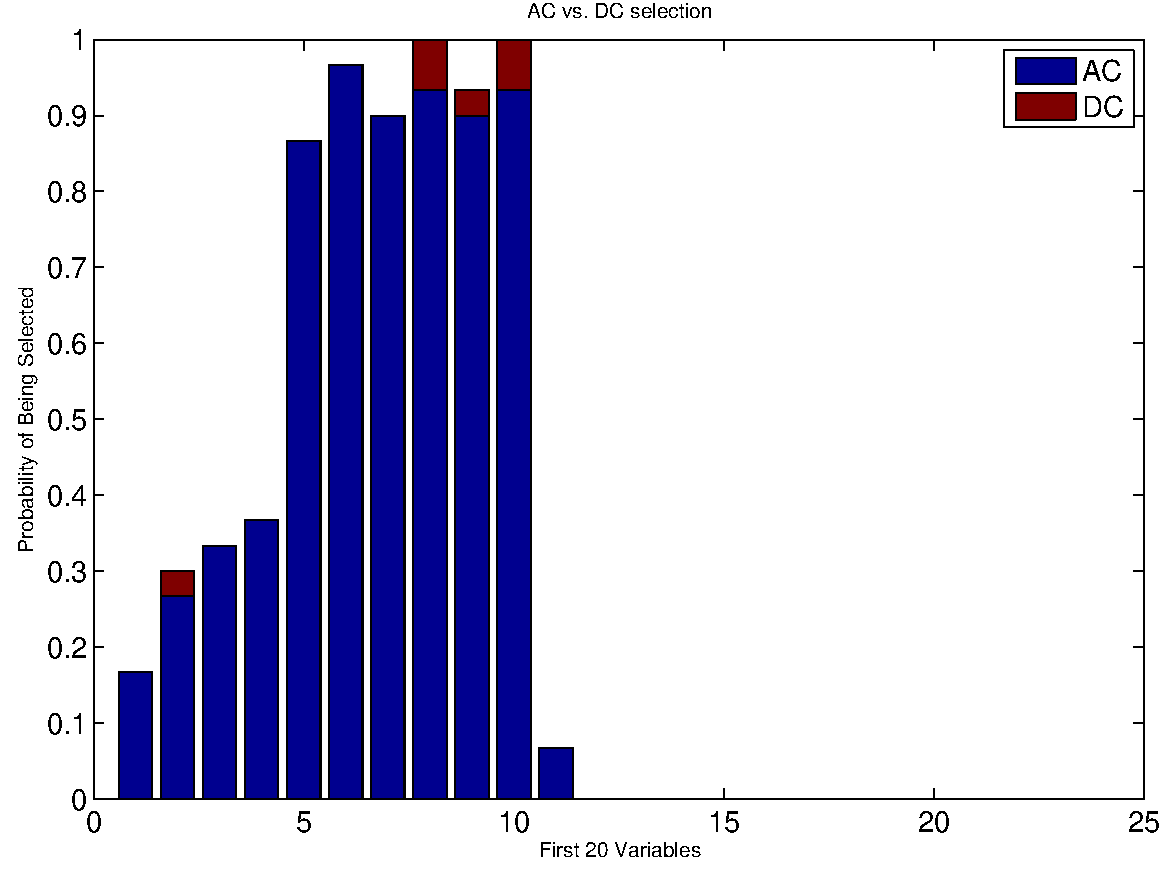
\includegraphics[width=0.5\textwidth]{figs/ACvDC}
\caption{Frequency of variable selection among the first 20 variables ($X_j$ for $j=1,...,20$) in the AC stage vs. in the DC stage. The true variables are [5,6,7,8,9,10].}
\label{fig:ac_v_dc}
\end{figure*}


\subsection{Boston housing data}

We next use the Boston housing data rather than simulated data. This data set
contains 13 covariates, 506 samples and one response variable
indicating housing values in suburbs of Boston. The data and detailed description
can be found on the UCI Machine Learning Repository website\footnote{\url{http://archive.ics.uci.edu/ml/datasets/Housing}}. 

We first use all $n=506$ samples (with standardization) in the AC/DC algorithm,
using a set of candidate regularization parameters $\{\lambda^{(t)}\}$
ranging from $\lambda^{(1)} = 0$ (no regularization) to $2$. For each $\lambda^{(t)}$
we obtain a function value matrix $\bds{f}^{(t)}$ with $p=13$
columns and $n=506$ rows. The non-zero columns in this matrix indicate the variables selected using $\lambda^{(t)}$.  

In Figure~\ref{Boston}(a), we plot on the $y$-axis the norm
$\|\bds{f}^{(t)}_j\|_{\infty}$ of every column $j$ against the
regularization strength $\lambda^{(t)}$. Instead of plotting the value
of $\lambda^{(t)}$ on the $x$-axis,  however, we plot the total norm at
$\lambda^{(t)}$ normalized against the total norm at $\lambda^{(1)}$:
$\frac{\sum_j \|\bds{f}^{(t)}_j\|_{\infty}}{\sum_j
  \|\bds{f}^{(1)}\|_{\infty}}$. Thus, as $x$ moves from 0 to 1, the
regularization goes from strong to weak. For comparison, we plot the
LASSO/LARS result in a similar way in Figure \ref{Boston}(b).  From
the figures we observe that the first three variables selected by
AC/DC and LASSO are the same: \tts{LSTAT}, \tts{RM} and \tts{PTRATIO},
consistent with previous findings~\citep{SpAM:07}.  The fourth
variable selected by AC/DC is \tts{INDUS} (with $\lambda^{(t)}=0.7$).
We then refit AC/DC with only these four variables without
regularization, and plot the estimated additive functions in Figure
\ref{Boston}(d). When refitting, we constrain a component to be convex
if it is non-zero in the AC stage and concave if it is non-zero in the
DC stage. As can be seen, these functions contain clear nonlinear
effects which cannot be captured by LASSO. The shapes of these
functions, including the concave shape of the \tts{PTRATIO} function,
are in agreement with those obtained by SpAM~\citep{SpAM:07}.

Next, in order to quantitatively study the predictive performance, we
run 3 times 5-fold cross validation, following the same procedure
described above---training, variable selection and refitting.  A plot
of the mean and standard deviation of the predictive mean squared
error (MSE) is shown in Figure \ref{Boston}(c). Since for AC/DC the same
regularization level $\lambda^{(t)}$ may lead to a slightly different number of selected
variables in different folds and runs, the values on the $x$-axis
for AC/DC are not necessarily integers. The figure clearly shows that AC/DC has a 
lower predictive MSE than LASSO.  We also compared the performance of
AC/DC with that of Additive Forward Regression (AFR) presented
in~\cite{Xi:09}, and found that they are similar.  The main advantages
of AC/DC compared with AFR and SpAM are that there are no smoothing
parameters required, and the optimization is formulated
as a convex program, guaranteeing a global optimum.

%\begin{figure}[!htpb]
%        \centering
%        \begin{subfigure}[b]{0.45\textwidth}
%                \centering
%                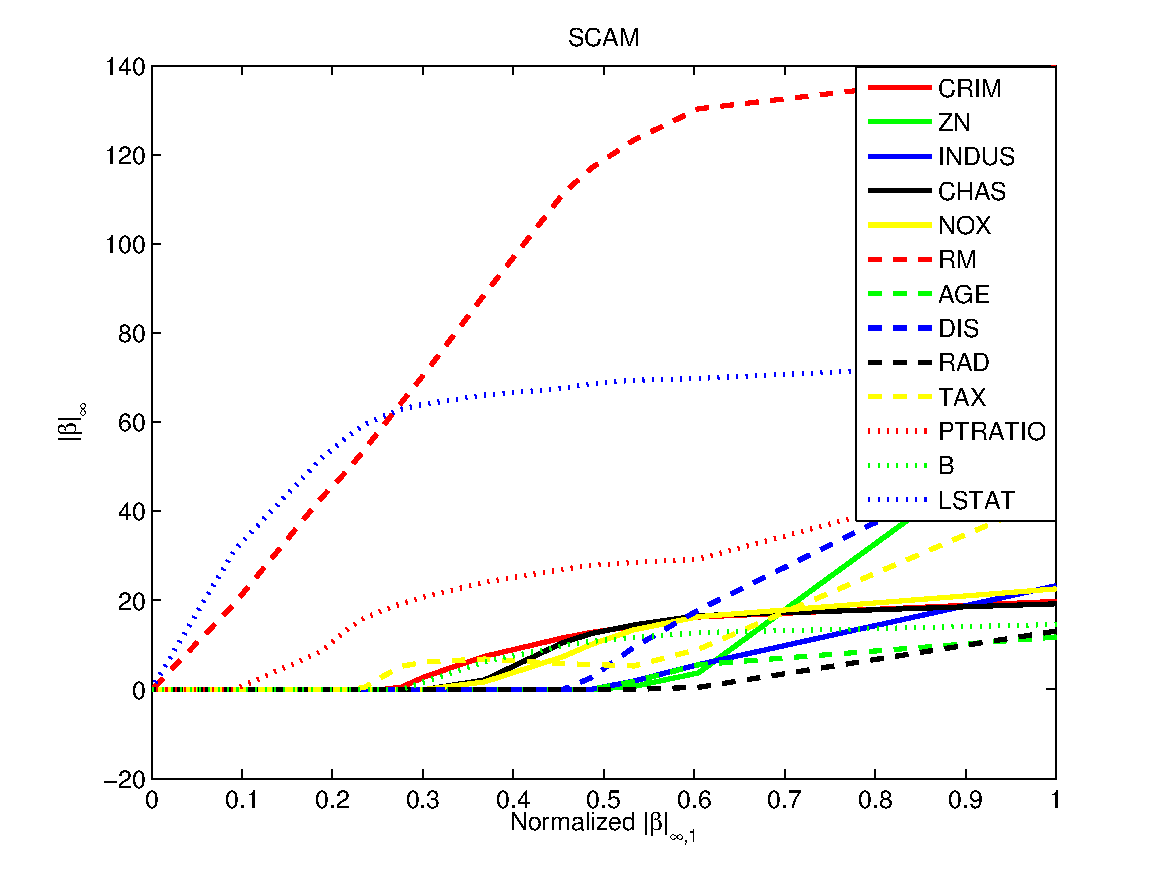
\includegraphics[width=\textwidth]{figs/Additive}
%                 \caption{Variable selection result using AC/DC.}
%                \label{AC/DC}
%        \end{subfigure}
%        \begin{subfigure}[b]{0.45\textwidth}
%                \centering
%                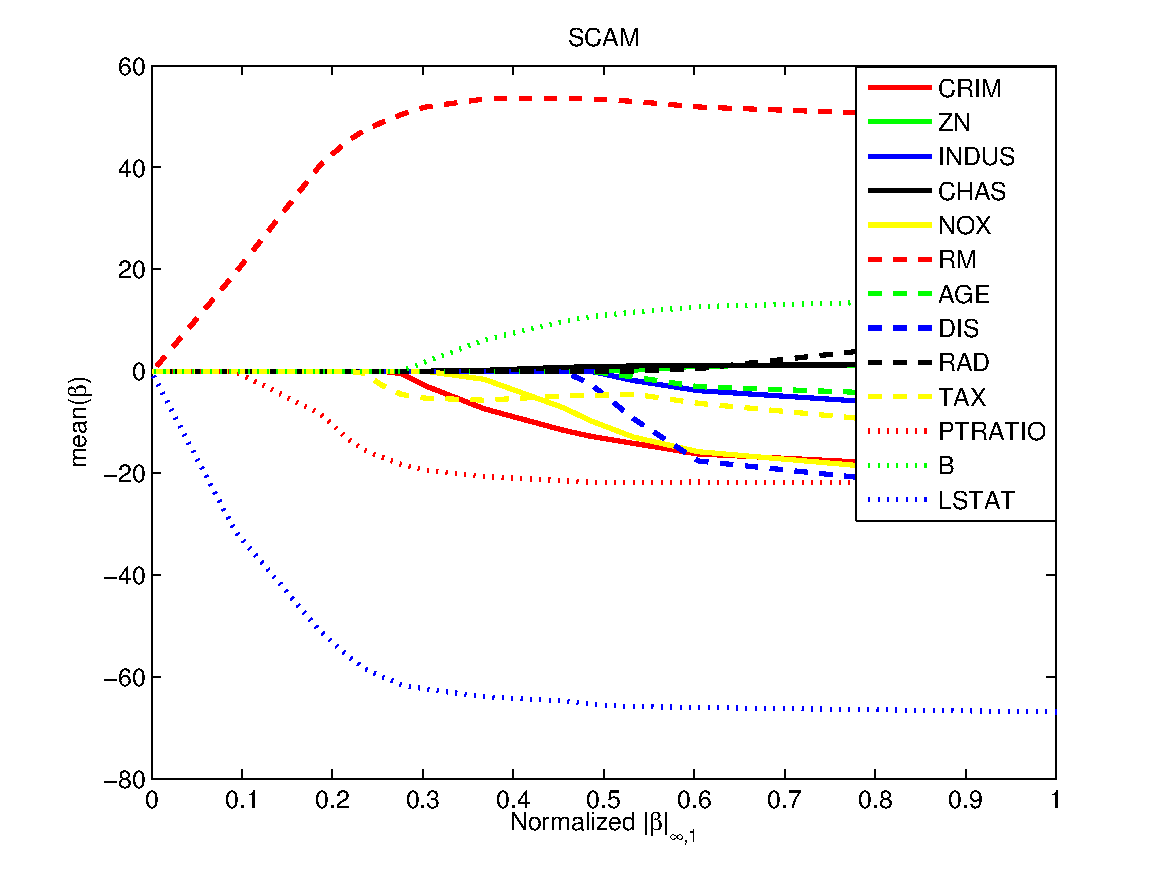
\includegraphics[width=\textwidth]{figs/Additive1}
%                 \caption{Variable selection result using AC/DC.}
%                \label{AC/DC1}
%        \end{subfigure}\\
%        \begin{subfigure}[b]{0.45\textwidth}
%                \centering
%                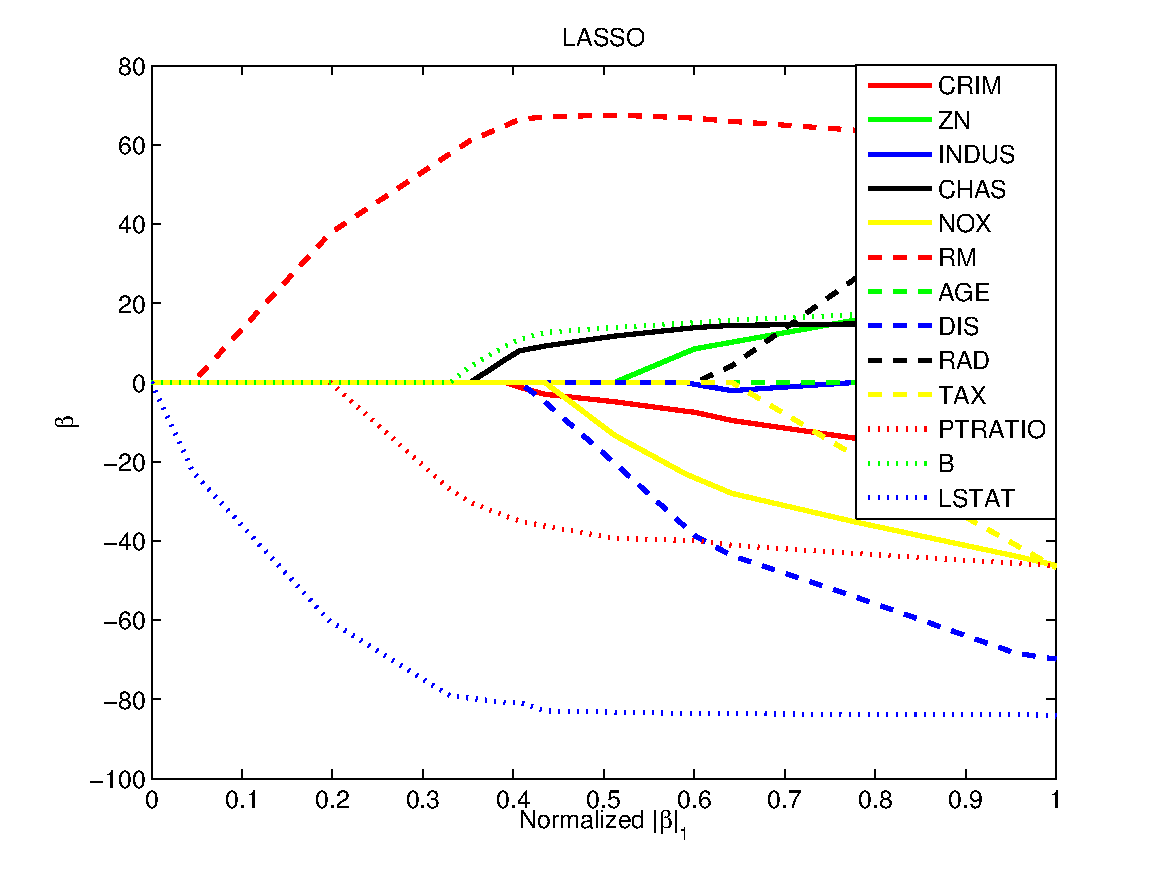
\includegraphics[width=\textwidth]{figs/LASSO}
%                \caption{Variable selection result using LASSO.}
%                \label{LASSO}
%        \end{subfigure}
%        \begin{subfigure}[b]{0.45\textwidth}
%                \centering
%                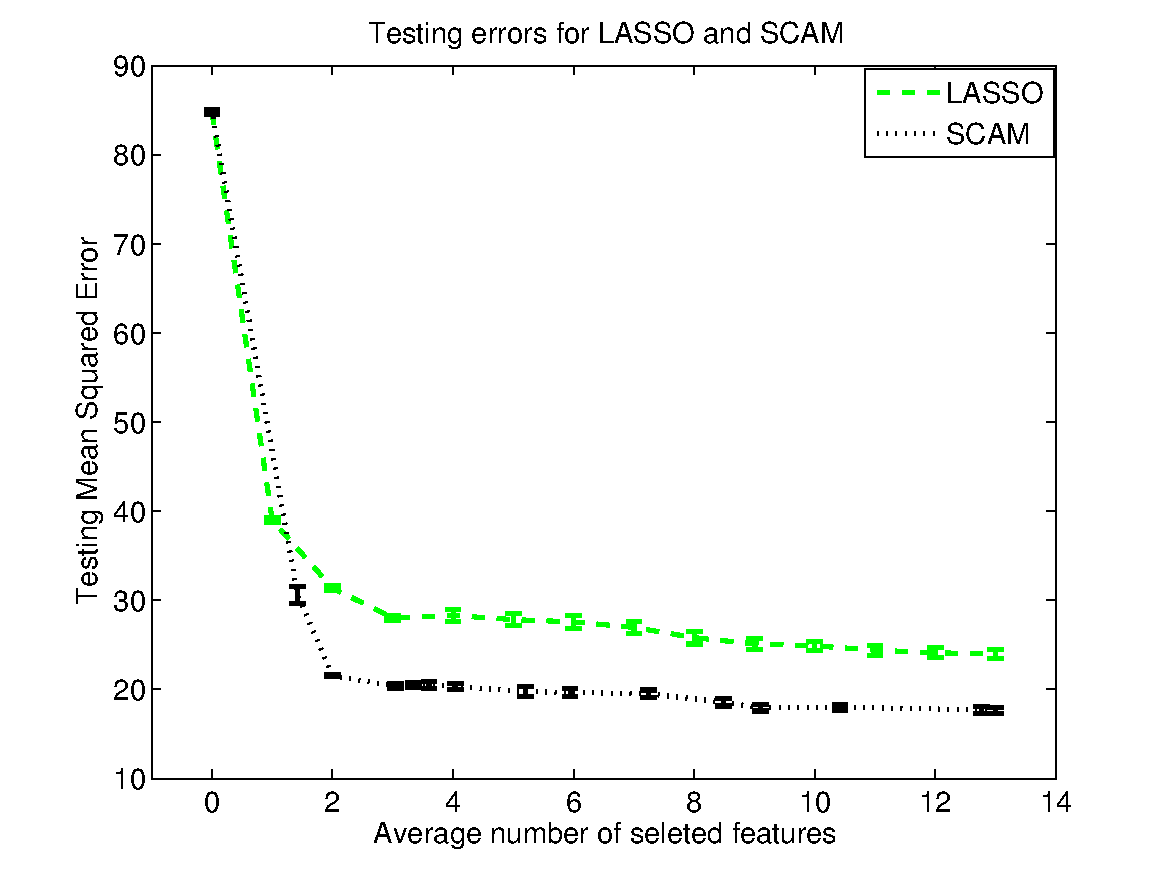
\includegraphics[width=\textwidth]{figs/MSE}
%                 \caption{Predictive MSE of AC/DC and LASSO.}
%                 \label{MSE}
%        \end{subfigure}\\
%        \begin{subfigure}[b]{0.45\textwidth}
%                \centering
%                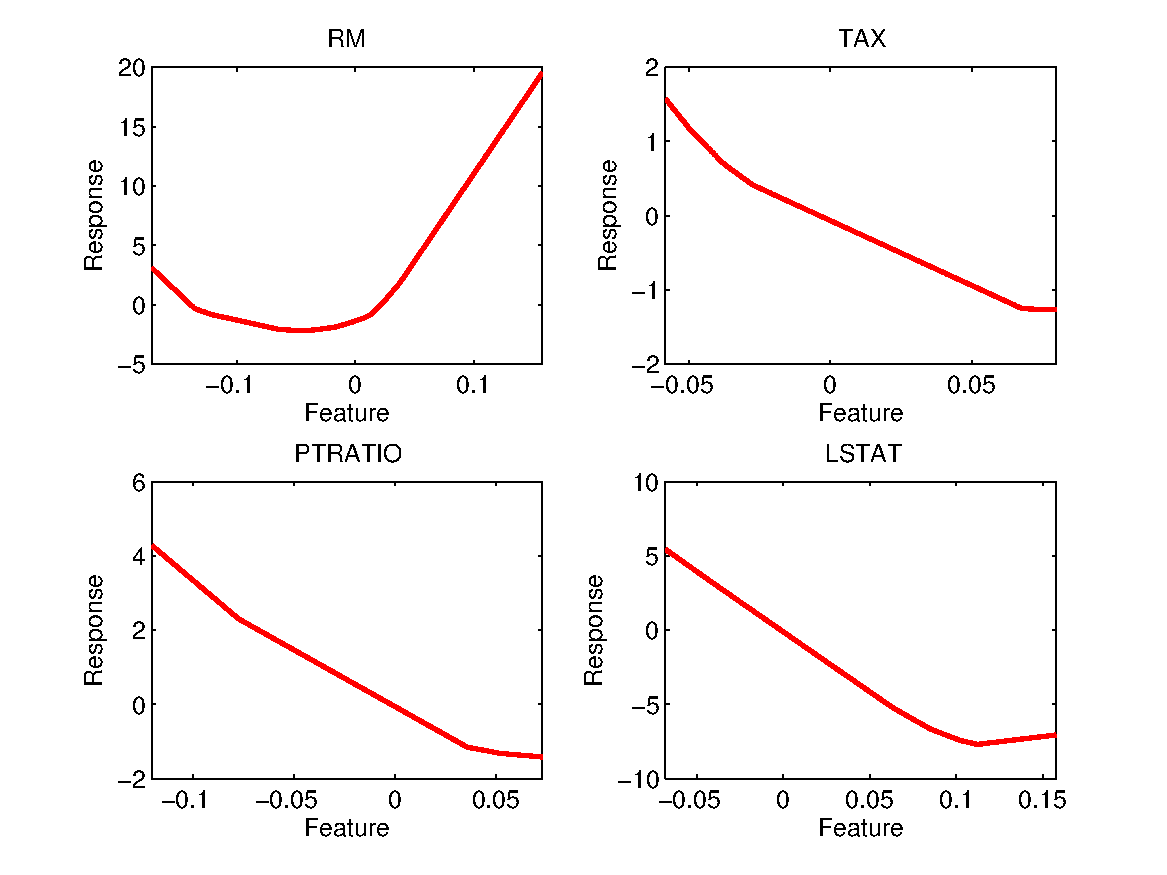
\includegraphics[width=\textwidth]{figs/Convex}
%                \caption{Inferred additive convex functions by AC/DC.}
%                \label{Convex}
%        \end{subfigure}
%        \caption{Results on Boston housing data.}\label{Boston}
%\end{figure}



\begin{figure*}[t]
\begin{center}
\begin{tabular}{cc}
%\hskip-10pt
  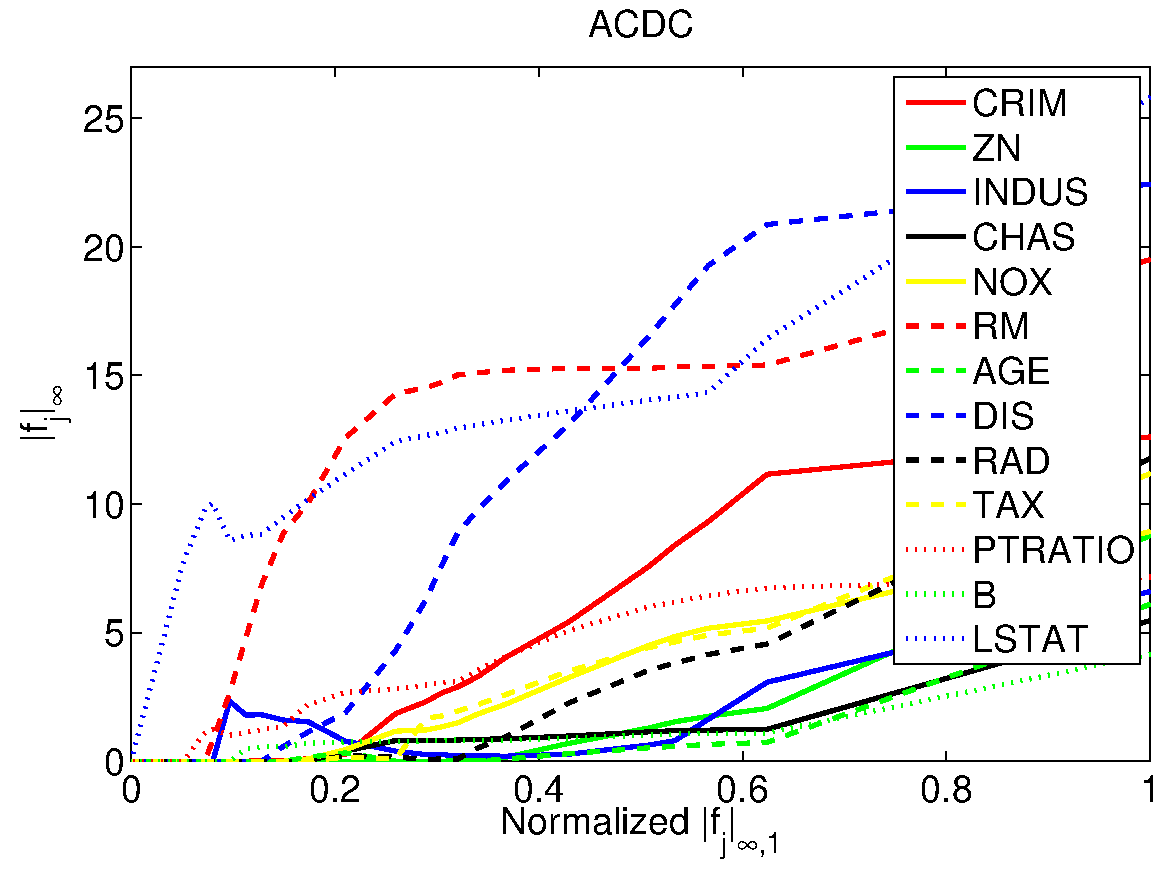
\includegraphics[width=.38\textwidth]{figs/acdc_path}  &
%\hskip-25pt
  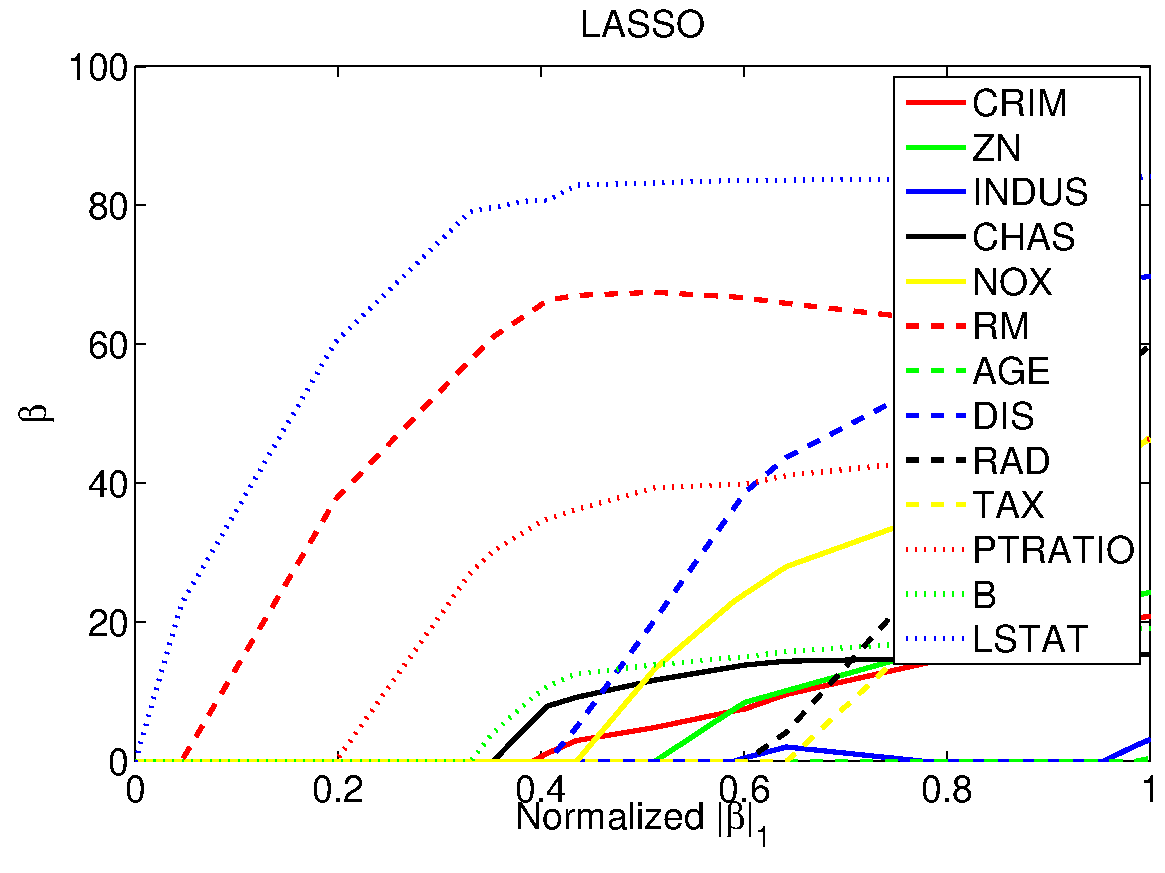
\includegraphics[width=.38\textwidth]{figs/lasso_path} 
\\
%\hskip-10pt 
(a) AC/DC $\|f_k\|_\infty$ paths & 
%\hskip-25pt
(b) LASSO $|\beta_k|$ paths \\
%\end{tabular}
%\begin{tabular}{cc}
  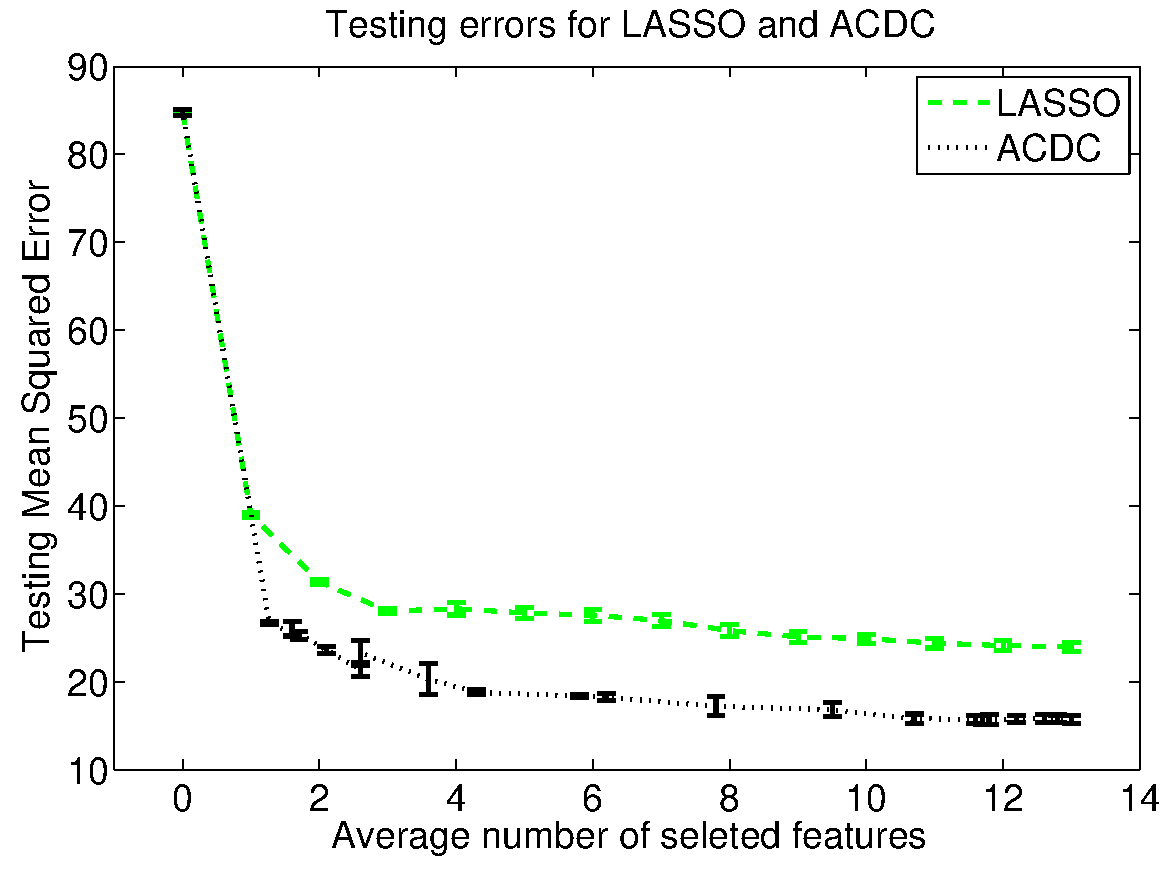
\includegraphics[width=.38\textwidth]{figs/MSEacdc} &
%\hskip 5pt
  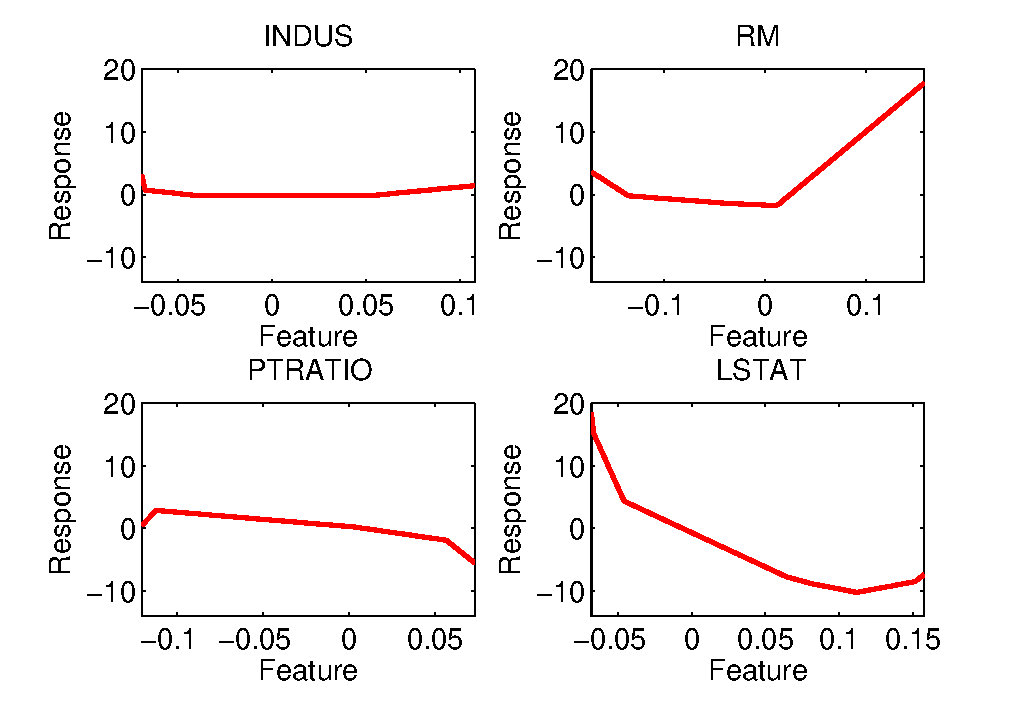
\includegraphics[width=.45\textwidth]{figs/acdc_functs}
\\
(c) predictive MSE & (d) estimated functions from AC/DC
\end{tabular}
\end{center}
\caption{Results on Boston housing data, showing regularization paths,
 MSE and fitted functions.} \label{Boston}
\end{figure*}


% DO NOT CHANGE; RefTex variables -minx
 
%%% Local Variables: ***
%%% mode:latex ***
%%% TeX-master: "paper-submit.tex" ***
%%% End: ***

